\documentclass[12pt]{scrartcl}


\usepackage{epsfig,amssymb}

\usepackage{xcolor}
\usepackage{graphicx}
\usepackage{epstopdf}
\usepackage{multirow}

\definecolor{darkred}{rgb}{0.5,0,0}
\definecolor{darkgreen}{rgb}{0,0.5,0}
\usepackage[pdfusetitle]{hyperref}
\hypersetup{
  letterpaper,
  colorlinks,
  linkcolor=red,
  citecolor=darkgreen,
  menucolor=darkred,
  urlcolor=blue,
  pdfpagemode=none,
}

\usepackage{fullpage}
\usepackage{tikz}
\pagestyle{empty} %
\usepackage{subfigure}

\definecolor{MyDarkBlue}{rgb}{0,0.08,0.45}
\definecolor{MyDarkRed}{rgb}{0.45,0.08,0}
\definecolor{MyDarkGreen}{rgb}{0.08,0.45,0.08}

\definecolor{mintedBackground}{rgb}{0.95,0.95,0.95}
\definecolor{mintedInlineBackground}{rgb}{.90,.90,1}

\usepackage[newfloat=true]{minted}

\setminted{mathescape,
           linenos,
           autogobble,
           frame=none,
           framesep=2mm,
           framerule=0.4pt,
           %label=foo,
           xleftmargin=2em,
           xrightmargin=0em,
           %startinline=true,  %PHP only, allow it to omit the PHP Tags *** with this option, variables using dollar sign in comments are treated as latex math
           numbersep=10pt, %gap between line numbers and start of line
           style=default} %syntax highlighting style, default is "default"

\setmintedinline{bgcolor={mintedBackground}}
%doesn't work with the above workaround:
\setminted{bgcolor={mintedBackground}}
\setminted[text]{bgcolor={mintedBackground},linenos=false,autogobble,xleftmargin=1em}
%\setminted[php]{bgcolor=mintedBackgroundPHP} %startinline=True}
\SetupFloatingEnvironment{listing}{name=Code Sample}
\SetupFloatingEnvironment{listing}{listname=List of Code Samples}

\setlength{\parindent}{0pt} %
\setlength{\parskip}{.25cm}
\newcommand{\comment}[1]{}

\usepackage{amsmath}
\usepackage{algorithm2e}
\SetKwInOut{Input}{input}
\SetKwInOut{Output}{output}
%NOTE: you can embed algorithms in solutions, but they cannot be floating objects; use [H] to make them non-floats

\usepackage{lastpage}

%\usepackage{titling}
\usepackage{fancyhdr}
\renewcommand*{\titlepagestyle}{fancy}
\pagestyle{fancy}
%\fancyhf{}
%\rhead{Computer Science I}
%\lhead{Guides and tutorials}
\renewcommand{\headrulewidth}{0.0pt}
\renewcommand{\footrulewidth}{0.4pt}
\lfoot{\Title\ -- Computer Science I}
\cfoot{~}
\rfoot{\thepage\ / \pageref*{LastPage}}

%remove headers
\rhead{~}
\lhead{~}


\makeatletter
\title{Hack 1.0}\let\Title\@title
\subtitle{Computer Science I\\
{\small
\vskip1cm
Department of Computer Science \& Engineering \\
University of Nebraska--Lincoln}
\vskip-1cm}
%\author{Dr.\ Chris Bourke}
\date{~}
\makeatother

\begin{document}

\maketitle

\hrule

\section*{Introduction}

Hack session activities are small weekly programming assignments intended
to get you started on full programming assignments.  Collaboration is allowed
and, in fact, \emph{highly encouraged}.  You may start on the activity before
your hack session, but during the hack session you must either be actively 
working on this activity or \emph{helping others} work on the activity.
You are graded using the same rubric as assignments so documentation, style, 
design and correctness are all important.

%\subsection*{Rubric}
%\begin{table}[H]
%\begin{tabular}{ll}
%Category       & Point Value \\
%Style          & 2           \\
%Documentation  & 2           \\
%Design         & 5           \\
%Correctness    & 16          \\
%\textbf{Total} & \textbf{25}
%\end{tabular}
%\end{table}



\section*{Problem Statement}

An essential tool when developing software is a \emph{version control system}
(VCS).  As you develop software you will make changes, add features, fix bugs, etc.
and it is necessary to keep track of your changes and to ensure that your 
code and other artifacts are backed up and protected by being stored on a 
reliable server (or multiple servers) instead of just one machine.  

A \emph{version control system} allows you to ``check-in'' or 
\emph{commit} changes to a code project.  It keeps track of all changes 
and allows you to ``branch'' a code base into a separate copy so that 
you can develop features or enhancements in isolation of the
main code base (often called the ``trunk'' in keeping with the tree 
metaphor).  Once a branch is completed (and well-tested and 
reviewed), it can then be \emph{merged} back into the main trunk 
and it becomes part of the project.

These systems are not only used for organizational and backup 
purposes, but are absolutely essential when developing software 
as part of a team.  Each team member can have their own working 
copy of the project code without interfering with other developer's 
copies or the main trunk.  Only when separate branches have to 
be merged into the trunk do conflicting changes have to be addressed.  
Such a system allows multiple developers to work on a 
very large and complex project in an organized manner.

\begin{figure}[h]
\centering
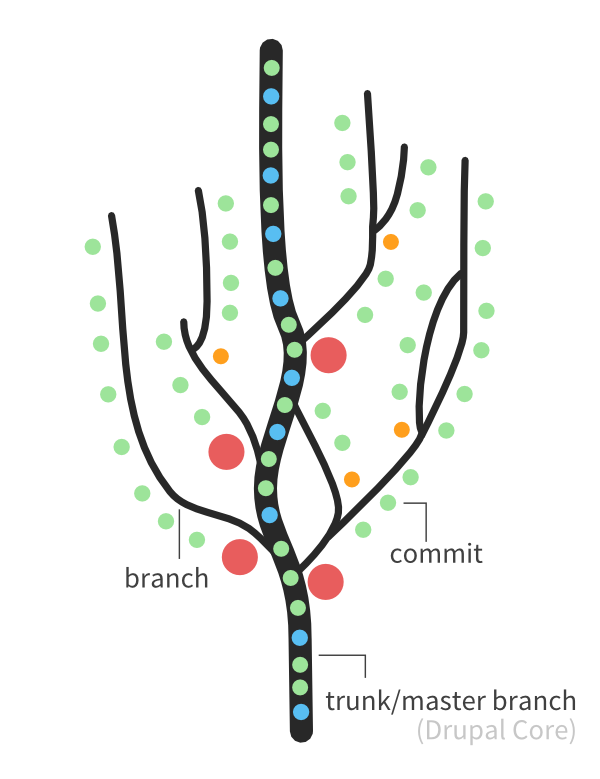
\includegraphics[scale=.5]{./hack1.0-files/repositorydiagram}
\caption{Trunk, branches, and merging visualization of the Drupal project}
\end{figure}

There are several widely used revision control systems including 
CVS (Concurrent Versions System), SVN (Apache Subversion), and 
Git.  SVN is a \emph{centralized} system: there is a single server that 
acts as the main code repository.  Individual developers can check out 
copies and branch copies (which are also stored in the main repository).  

Git is a \emph{distributed} VCS meaning that multiple servers/computers 
act as full repositories.  Each copy on each developer's machine 
\emph{also} contains a complete revision history.  This makes git a 
decentralized system.  Code commits are committed to a local repository.  
Merging a branch into another requires a push/pull request.  
Decentralizing the system means that anyone's 
machine can act as a code repository and can lead to wider collaboration 
and independence since different parties are no longer dependent on 
one master repository.

Git has become the de facto VCS system in software development.  We have
provided several external resources below, but this Hack will walk you
through the basics of getting started.  You will setup a project with 
git using GitHub (\url{https://github.com}) as your remote server.  You
will then collaborate with someone else to commit changes.

\section{Installation}

All of the instructions in this Hack will involve using GitHub's 
Desktop Client.  The screenshots were from the Mac version of this
program so it may look slightly different on other systems.  There 
are other alternatives and if you wish to use them you are welcome 
to do so.

\begin{enumerate}
  \item Go to \url{https://github.com/} and sign up/register with
  an account if you have not already done so.
  \item Download and the client here: \url{https://desktop.github.com/}.
\end{enumerate}

\section{Creating a Repository}

To focus on the git process, you will create and work with a simple
``Hello World''-style program but instead of printing ``Hello World'', 
it will print your name. 

\begin{enumerate}
  \item Create a new folder (call it \mintinline{text}{hello}) somewhere 
  on your computer and within it, 
  create a \mintinline{text}{hello.c} source file with code in it that
  prints your name.
  
  \item Open your GitHub Desktop Client (you may need to sign in with your
  new GitHub credentials).
  
  \item Drag and drop your \mintinline{text}{hello} folder to the GitHub Desktop
  Client.  It will look something like the following.
  \begin{center}
  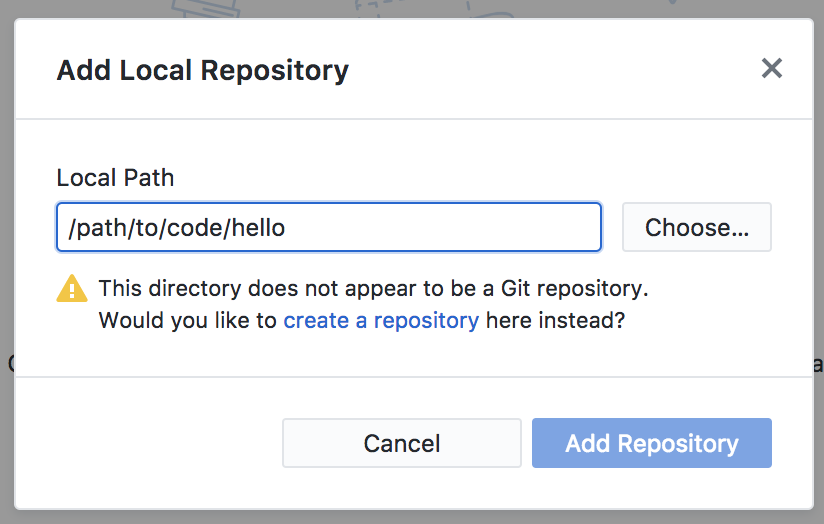
\includegraphics[scale=0.50]{./hack1.0-files/drag.png}
  \end{center}
  Click \mintinline{text}{create a repository} and it should look something
  like the following.
  \begin{center}
  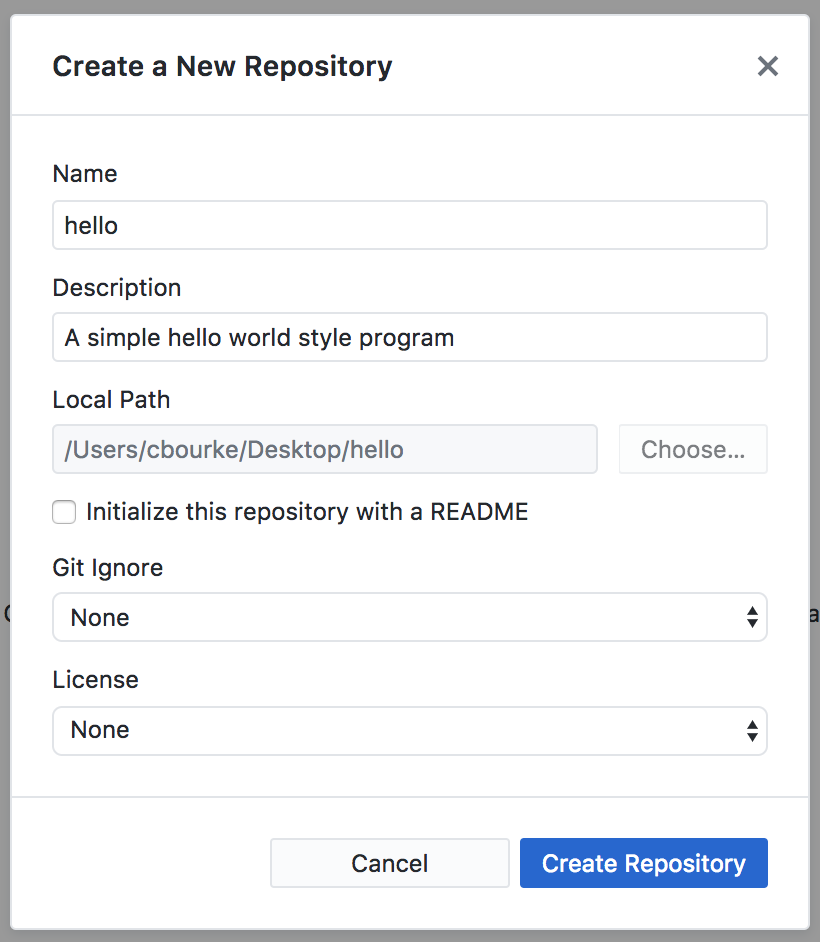
\includegraphics[scale=0.35]{./hack1.0-files/setup.png}
  \end{center}
  Provide a simple description and click \mintinline{text}{Create Repository}

  \item If everything is successful, it should look something like the following.
  \begin{center}
  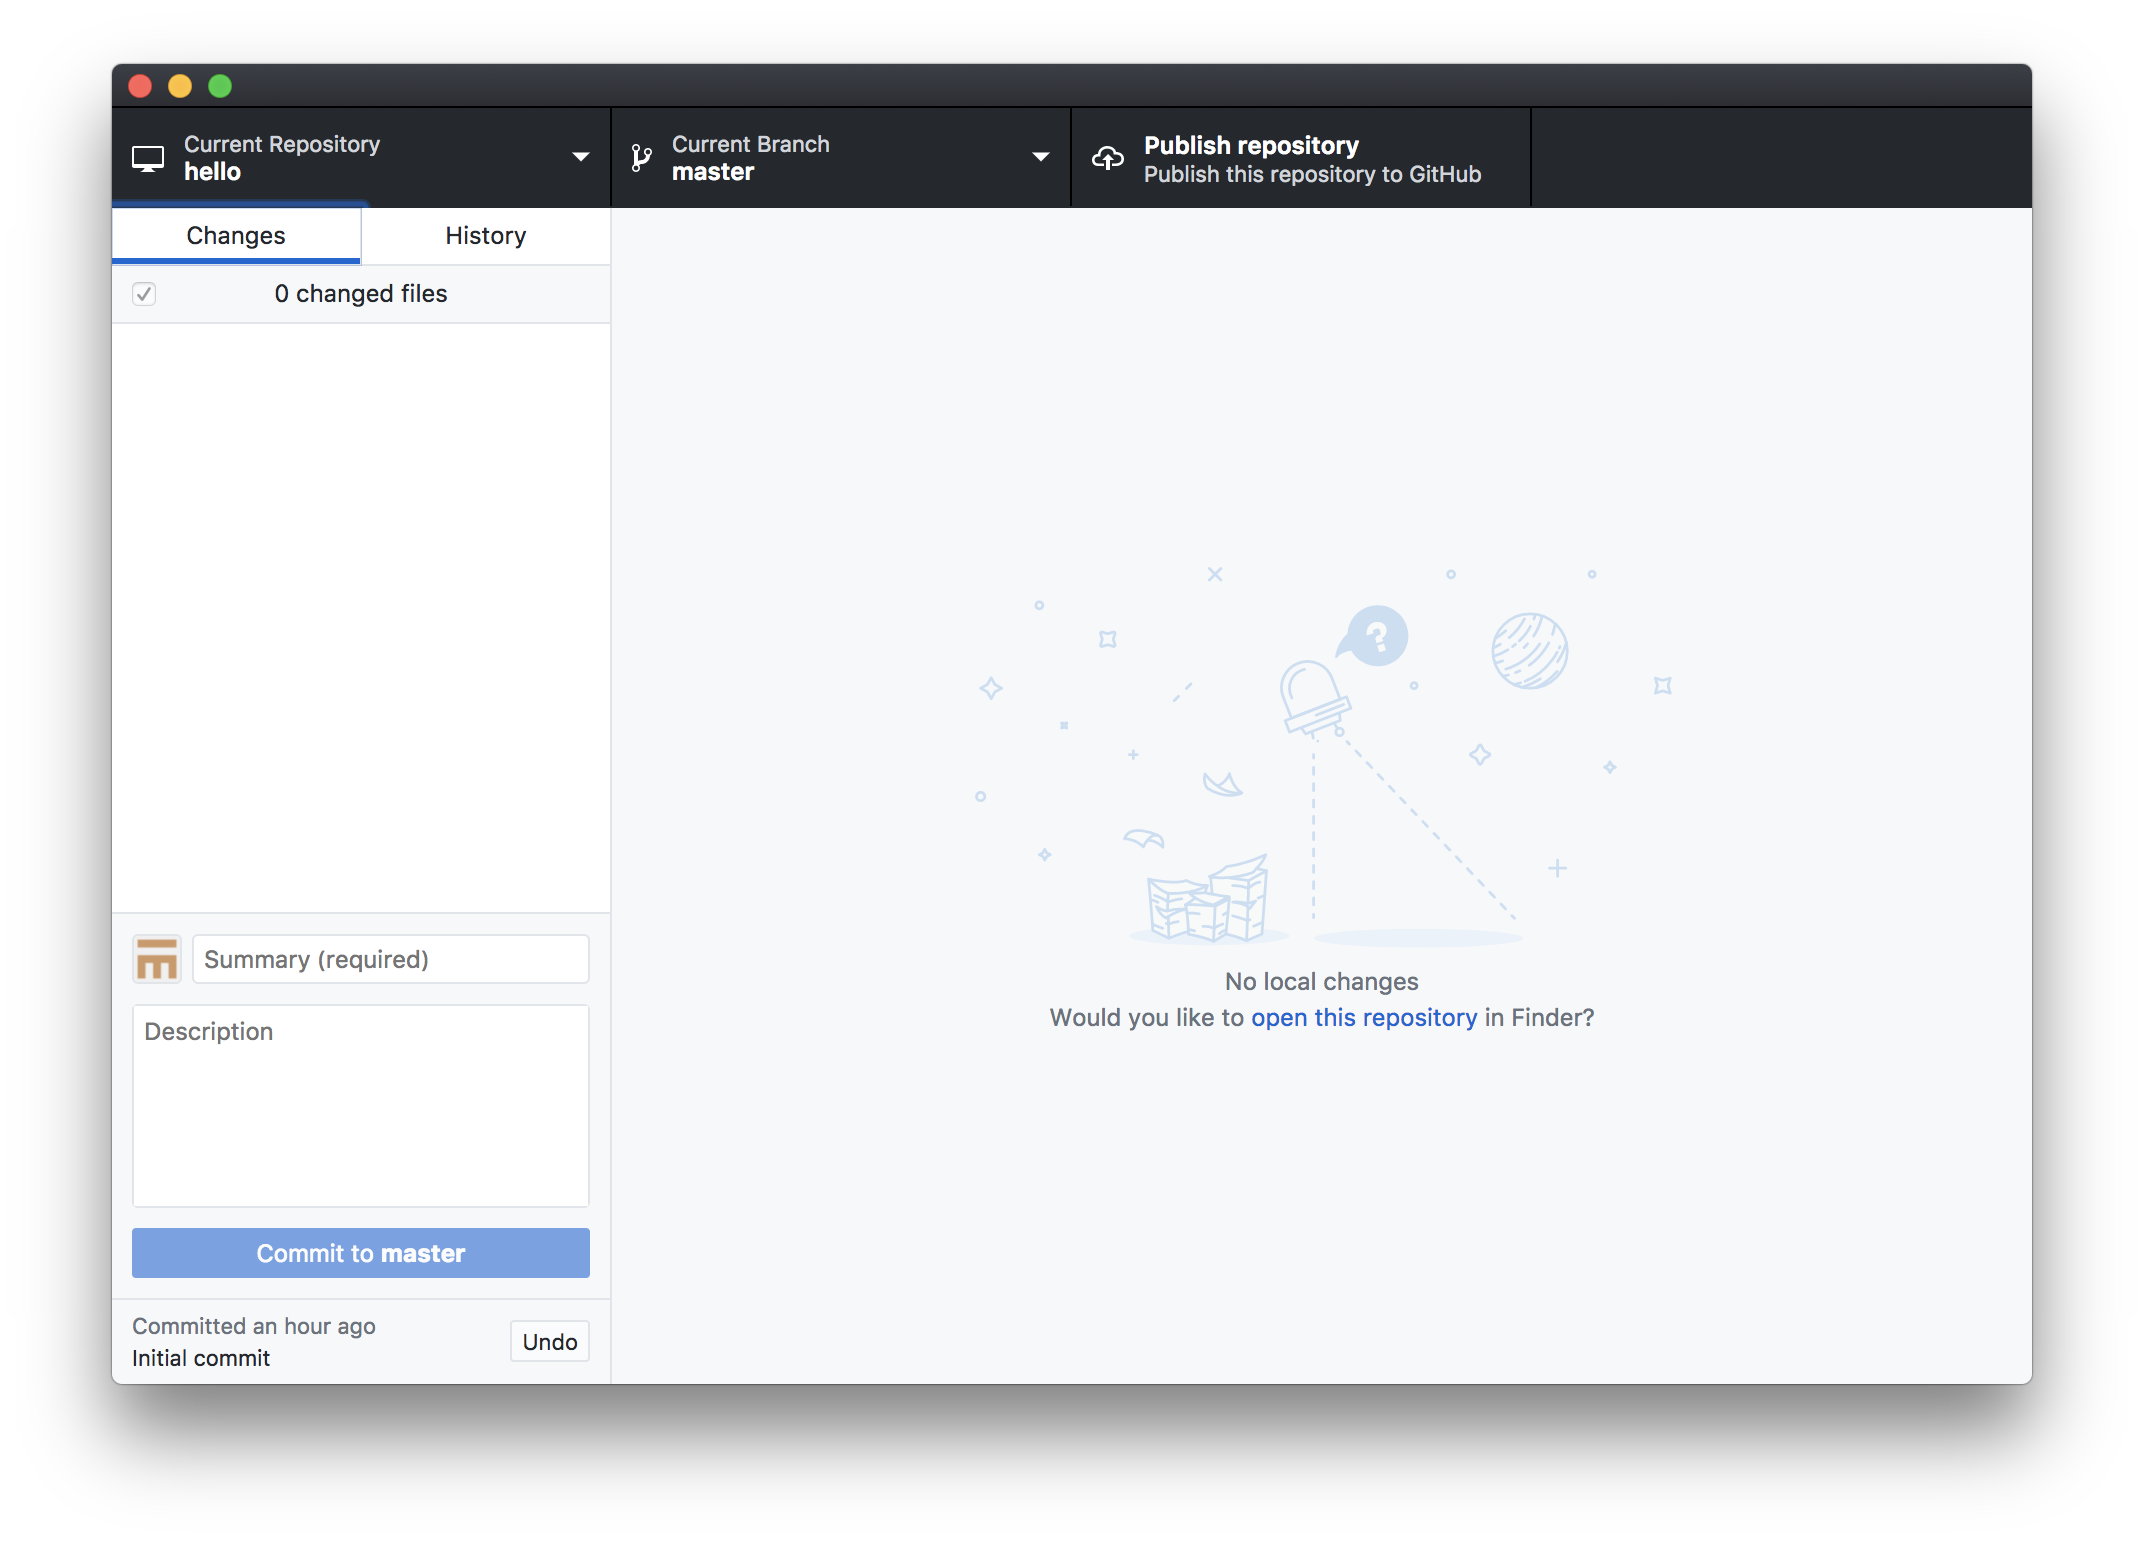
\includegraphics[scale=0.125]{./hack1.0-files/postCreation.png}
  \end{center}
  The GitHub client will have made an initial commit of the existing
  files for you.

  \item Push/publish your repository to GitHub.com by clicking 
  \mintinline{text}{Publish repository} at the top right.  It 
  should look look something like the following.  
  \begin{center}
  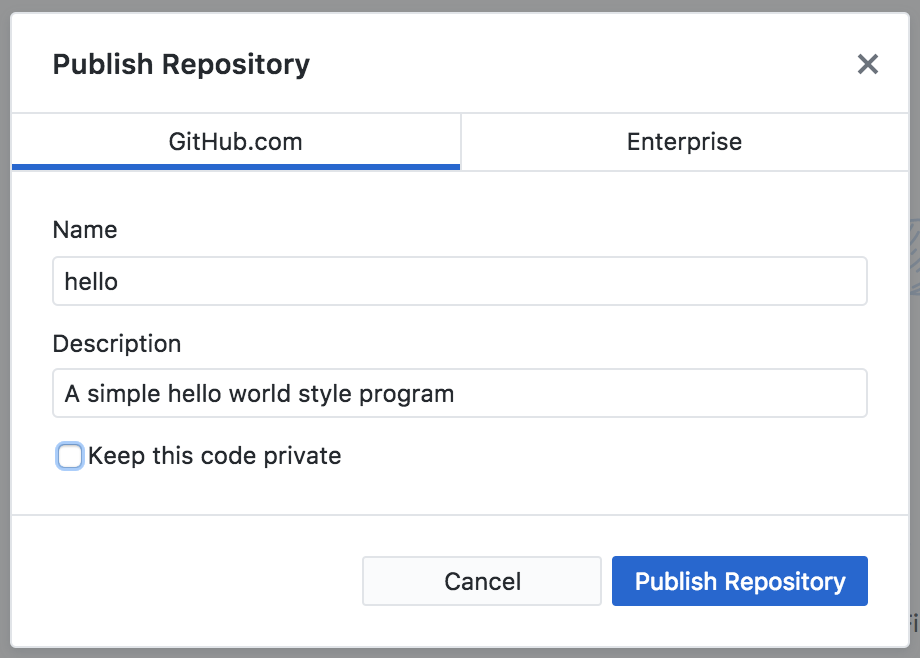
\includegraphics[scale=0.35]{./hack1.0-files/publish.png}
  \end{center}
  Be sure that \mintinline{text}{Keep this code private} is 
  \emph{not selected} and click \mintinline{text}{Publish Repository}
  
  \item If successful, your repository should now be on GitHub.
  Point your web browser to \url{https://github.com/login/hello}
  where \mintinline{text}{login} is replaced with your GitHub user
  name.  You can browse your repository, view its history, etc.
  
\end{enumerate}

\section{Making Changes}

You'll often make changes to you code that you should \emph{commit} to
your repository.  Though you may make changes and save them to a file, 
the changes are not saved to the repository's history.  Committing is 
the action that does this.  Committing only changes your \emph{local}
repository, the changes will still need to be \emph{pushed} to GitHub.
In this activity you'll make changes, commit them and then push them
to GitHub.

\begin{enumerate}
  \item Open the \mintinline{text}{hello.c} file and add a line that
  prints your major.  Be sure to save the file.

  \item The GitHub Client should ``see'' these changes.  It should look
  something like the following. 
  \begin{center}
  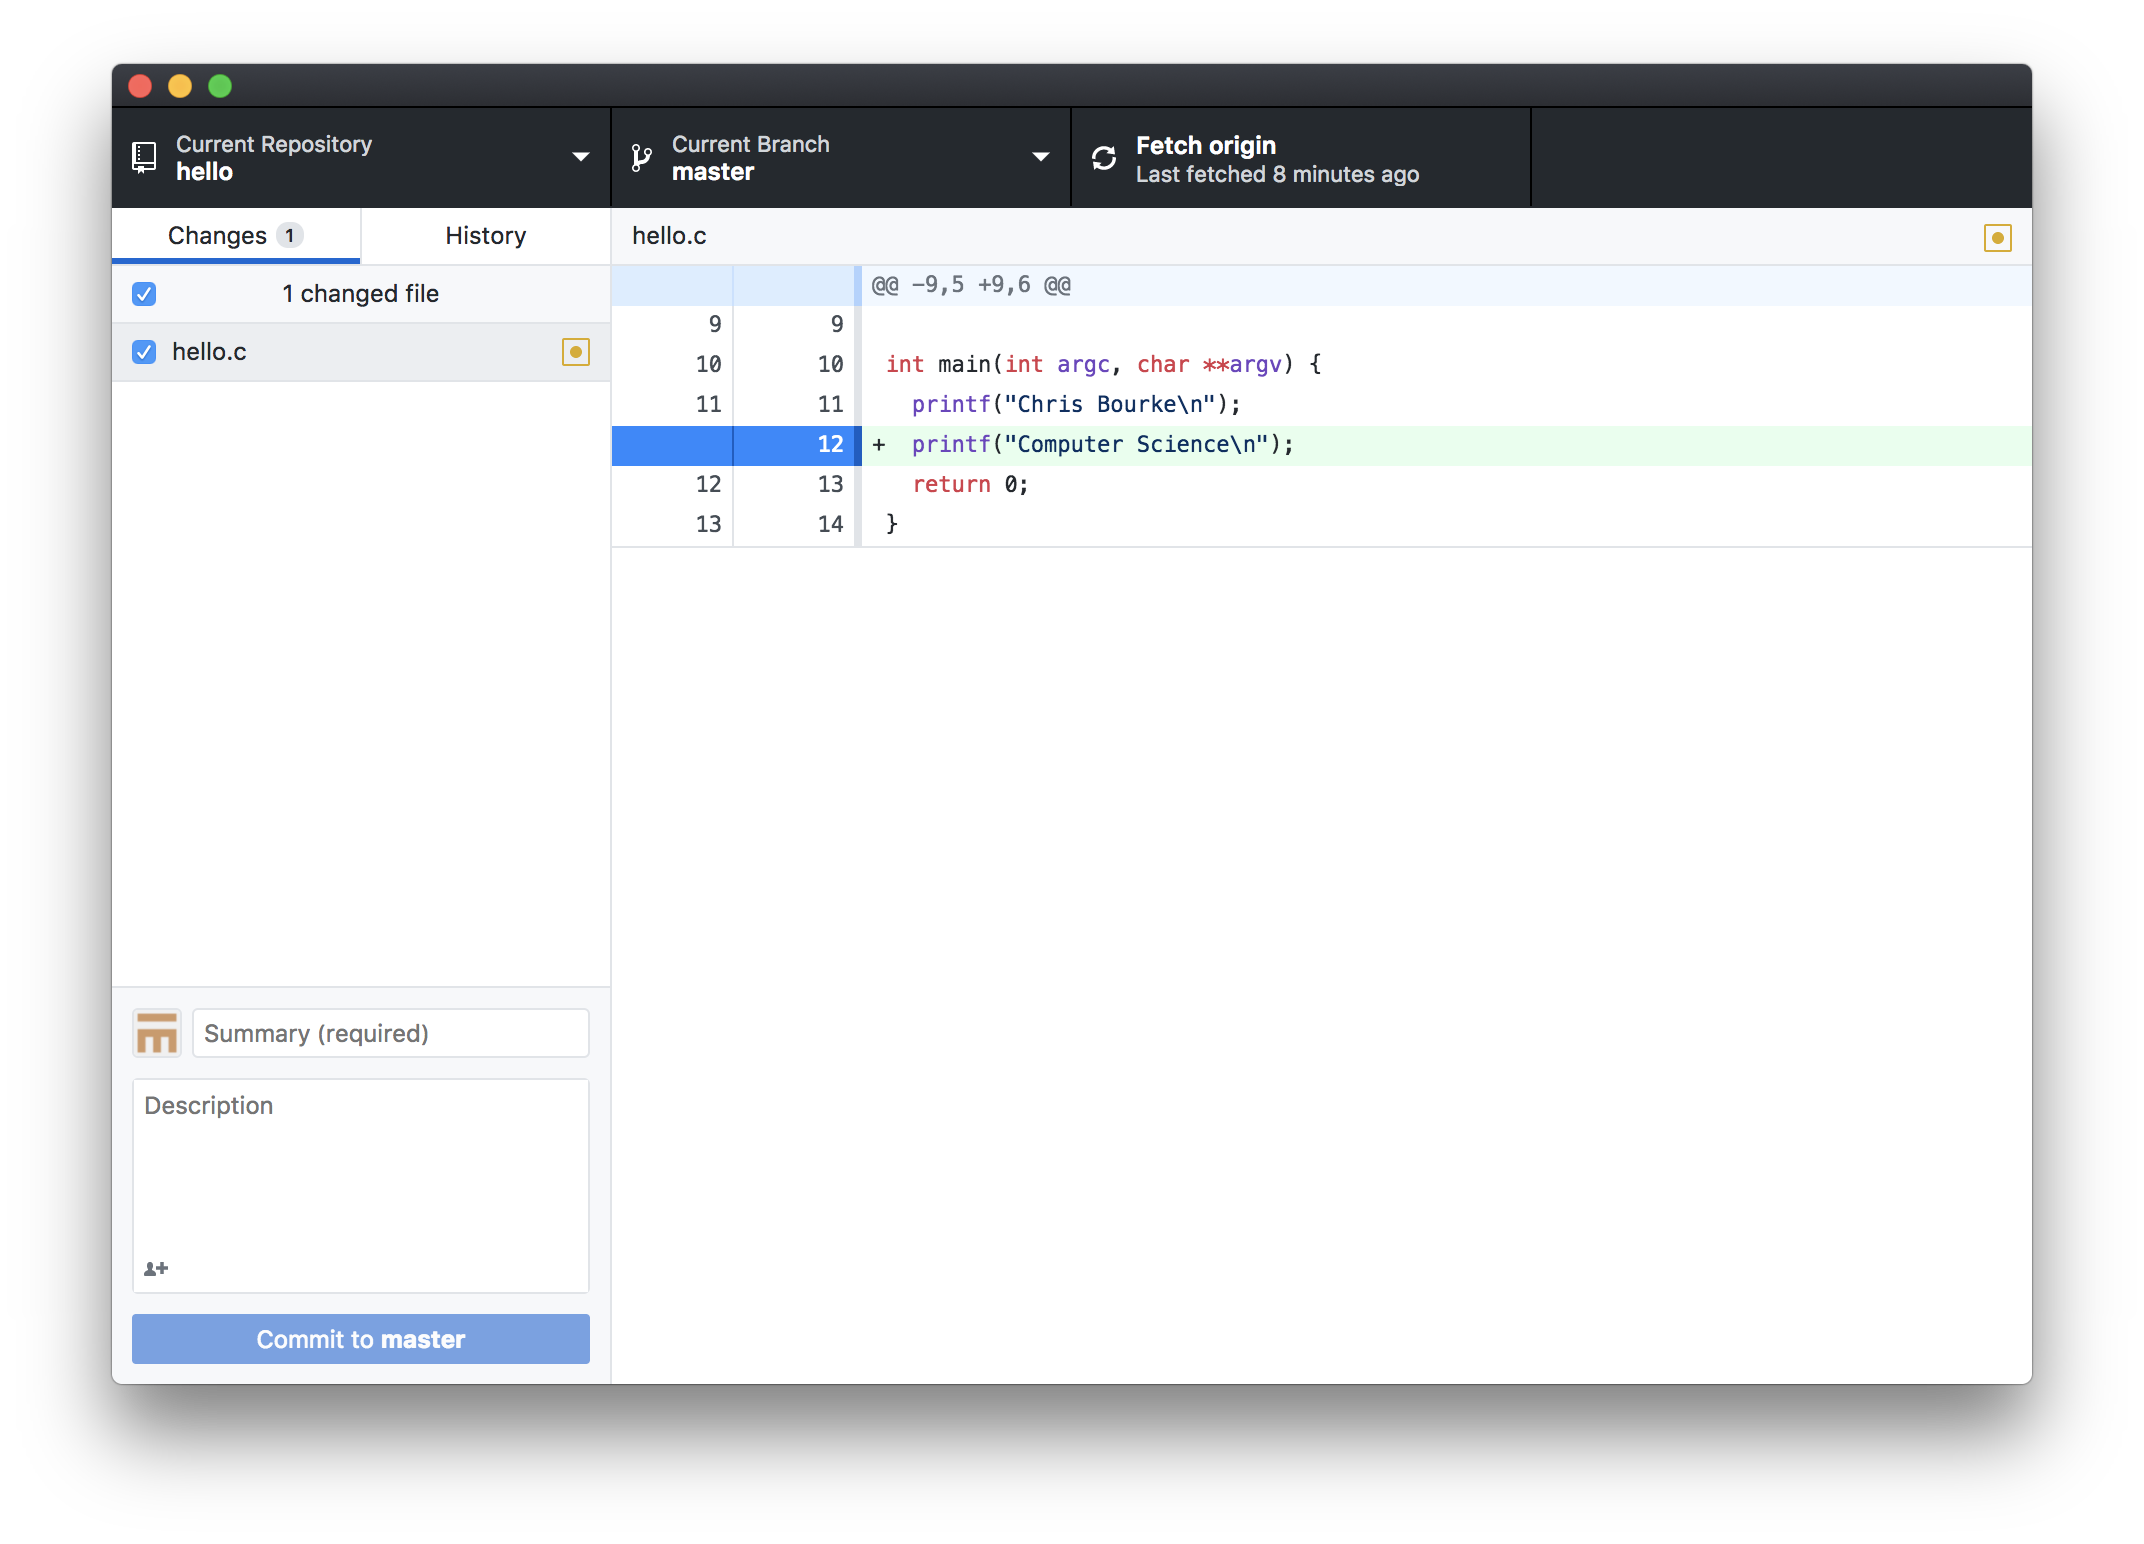
\includegraphics[scale=0.125]{./hack1.0-files/change.png}
  \end{center}

  \item Commit your changes by filling out the summary (required) and description.
  This is your chance to \emph{document} why you made changes to your code.
  Then click \mintinline{text}{Commit to master}.  Your changes have now
  been committed to your repository.  
  \begin{center}
  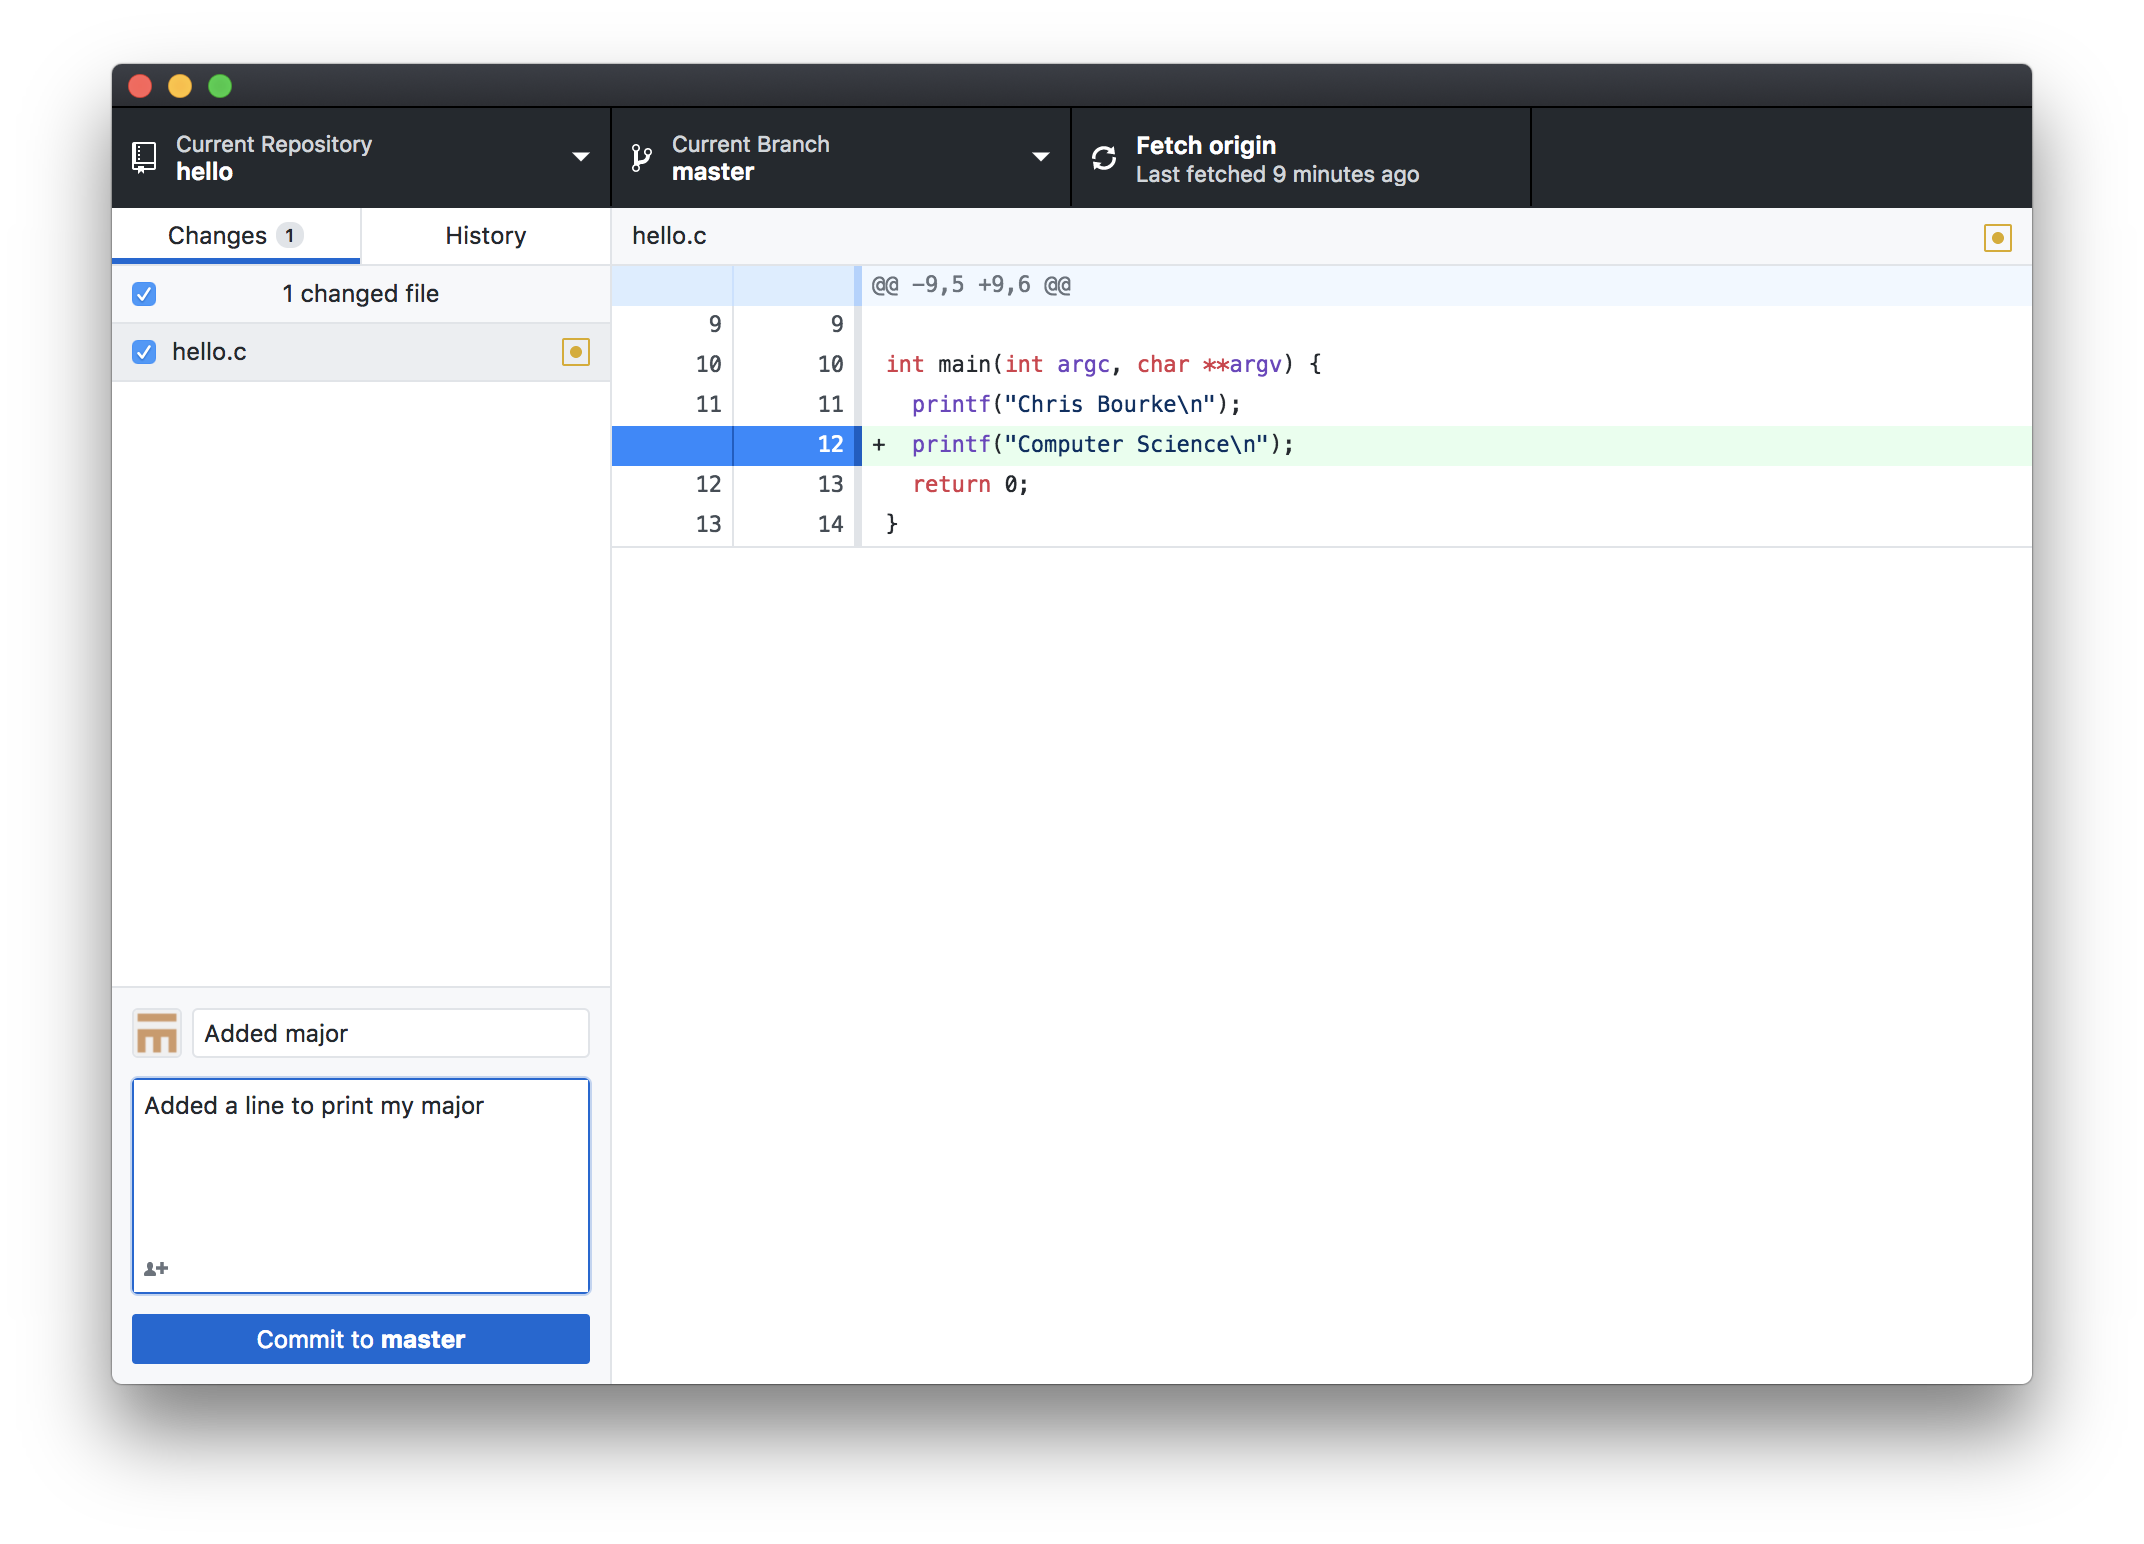
\includegraphics[scale=0.125]{./hack1.0-files/commit.png}
  \end{center}
  
  \item Push your changes to GitHub by clicking \mintinline{text}{Push origin}
  at the top right.  You can verify that your changes have been published
  to GitHub by refreshing your web browser.
  \begin{center}
  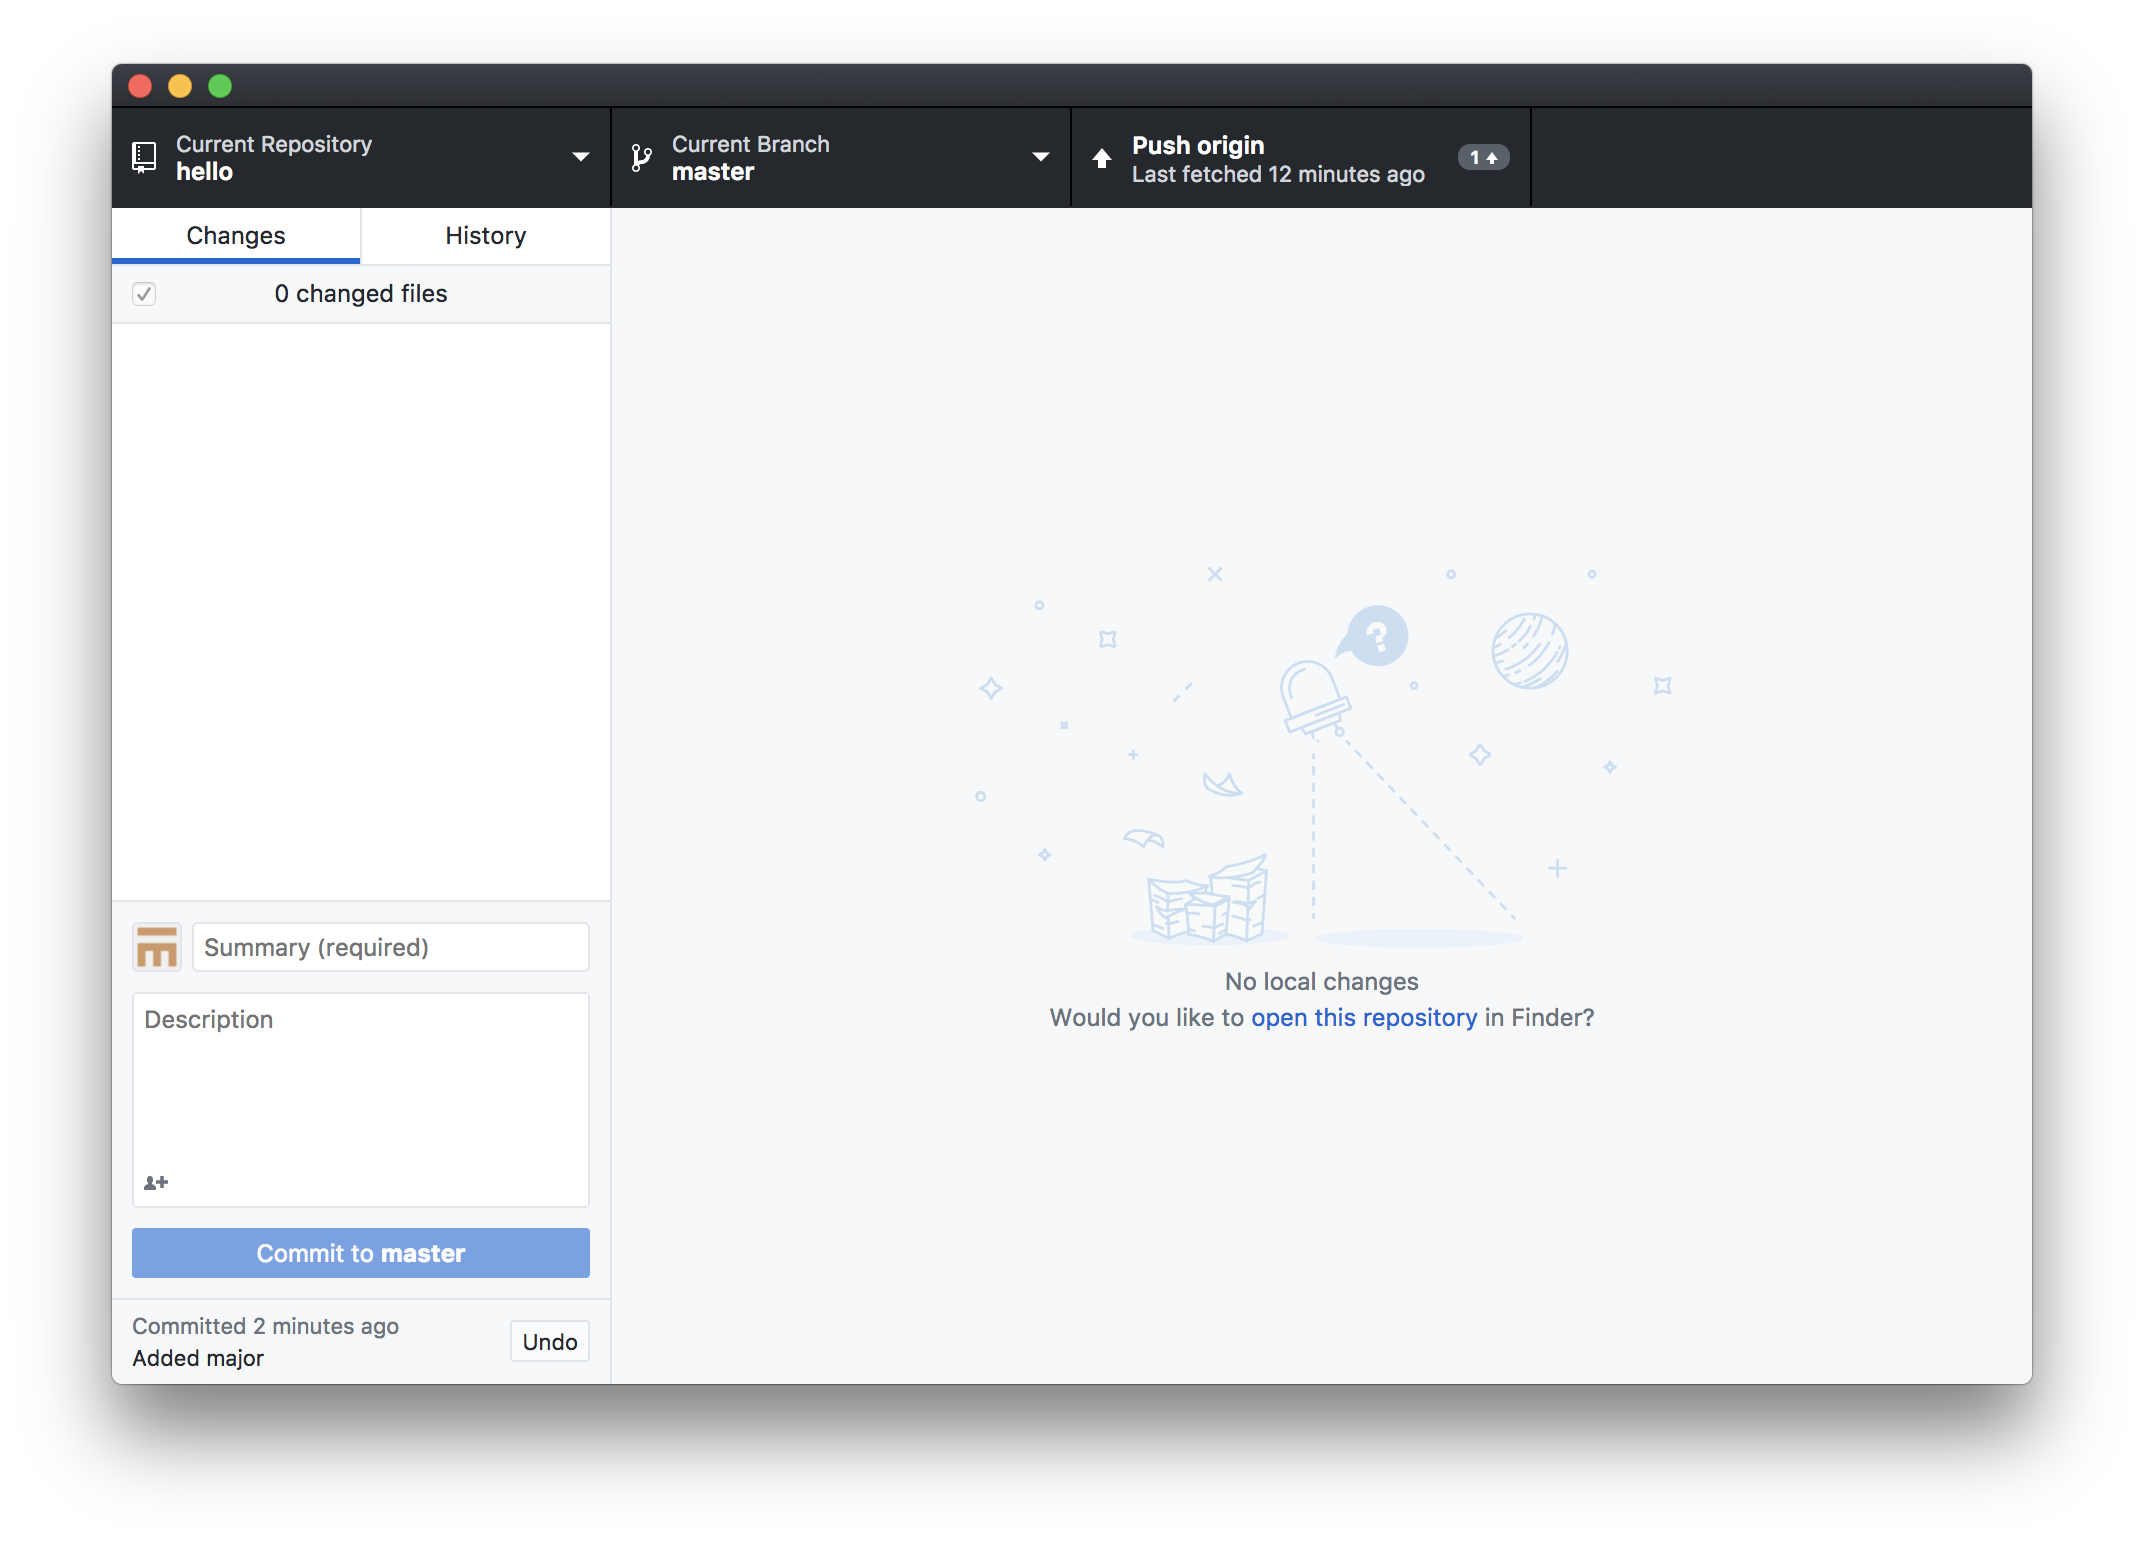
\includegraphics[scale=0.125]{./hack1.0-files/pushChange.png}
  \end{center}

\end{enumerate}

\section{Collaborating With a Team}

In this exercise, you'll need to team up with at least one other person.
You'll make them a collaborator on your project so they can make changes
and commit/push them to \emph{your} repository on GitHub.  Alternatively
you can have them make a pull request, but these instructions do not cover 
that; refer to one of the resources below for how how to make push/pull
requests.

\begin{enumerate}
  \item On GitHub.com, click \mintinline{text}{Settings} in your project.
  \item In the left menu, click \mintinline{text}{Collaborators}
  \item Type in your partner's GitHub user name and click \mintinline{text}{Add collaborator}
\end{enumerate}

\subsection{What your collaborator needs to do}

Together with your partner, walk through the following steps.  These
steps should be done on \emph{their} computer.

\begin{enumerate}
  \item Once you've sent an invite to collaborate, they need to accept it.
  \item Have them navigate their web browser to your GitHub 
  repository and click \mintinline{text}{Clone or download} and select
  \mintinline{text}{Open in Desktop}.  This will launch their GitHub
  Desktop Client and check out \emph{your} code.
  \item Have them add 2 lines of code to print their name and their major.
  \item In the GitHub Client, follow the same procedure to commit and push
  their changes to your repository using the same procedure as above.
  \item Verify their changes by refreshing your repository.  You can click
  on the \mintinline{text}{hello.c} and if you both did everything correctly, 
  you'll see multiple commits by multiple people:
  \begin{center}
  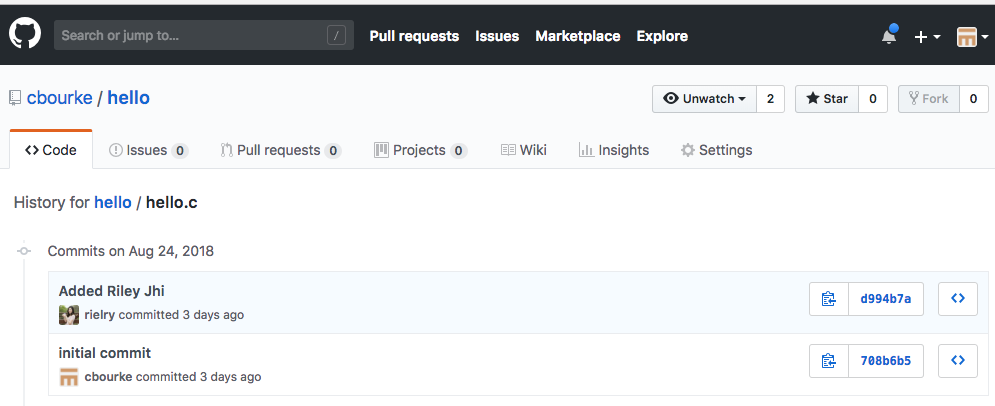
\includegraphics[scale=0.25]{./hack1.0-files/completedRepo02.png}
  \end{center}
  If you click on \mintinline{text}{History} you can see the changes for
  each commit: 
  \begin{center}
  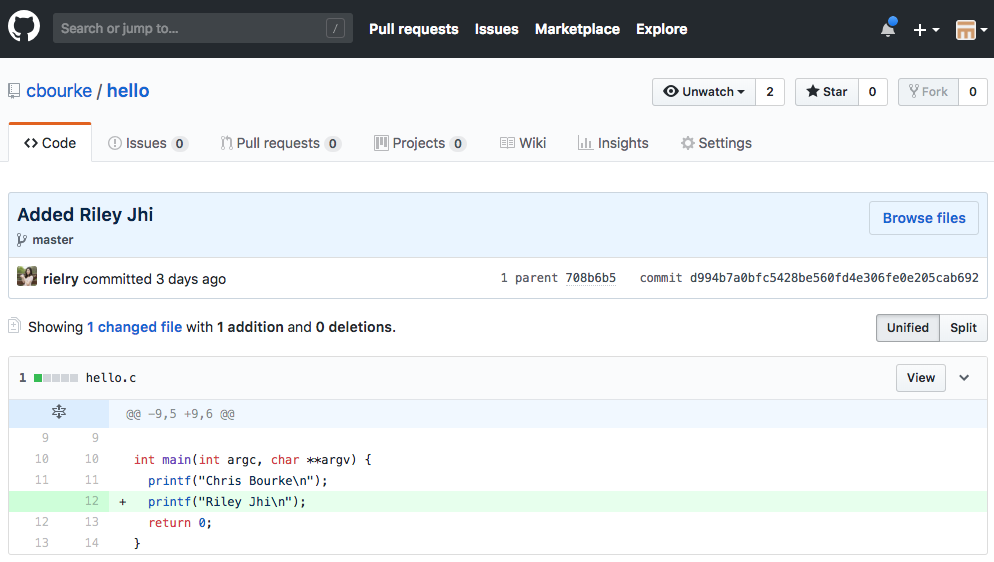
\includegraphics[scale=0.25]{./hack1.0-files/completedRepo03.png}
  \end{center}

\end{enumerate}

You are \emph{highly encouraged} to start using git/GitHub (or 
something similar) for all of your future assignments 
but be sure to commit code to a \emph{private} repository 
so that you do not violate the department's academic integrity 
policy.  

\subsection{Finishing Up}

\begin{enumerate}
  \item Put \emph{your} GitHub URL into a plain text file named 
  \mintinline{text}{readme.md}.  Turn this file
  in using webhandin.  Each individual student will need
  to hand in their own copy and will receive their own individual
  grade.
  \item Verify what you handed in by running the webgrader which will
  display the contents of your file.
\end{enumerate}


\section*{Additional Instructions}

\begin{itemize}
  \item You are encouraged to collaborate with any number of students 
  before, during, and after your scheduled hack session.    
  \item Each student is responsible for \emph{their} repository, so 
  if/when you team up with a partner, you'll need to go through this
  Hack at least twice: once as the primary repository owner and once as
  a collaborator.
\end{itemize}
  
\section*{Additional Resources}

\begin{itemize} 
  \item Video tutorial on Github Desktop: \url{https://www.youtube.com/watch?v=kFix7UDJ7LA}
  \item Interactive git tutorial: \url{https://try.github.io/levels/1/challenges/1}
  \item Pro Git, free online book: \url{https://git-scm.com/book/en/v2}
\end{itemize}


  


\end{document}
